%接線に関する参考資料
%\documentclass{jsarticle} \usepackage{graphics} \usepackage{amsmath} \usepackage{amssymb} \usepackage{cases}
%\newcommand{\pt}{$(x_1,y_1)$}

%\begin{document}
    \section{放物線}
    \subsection{導出}
    以下の放物線の\pt における接線を求める。
    \begin{equation}
        \label{eq:1-1}
        y=ax^2+ bx +c \hspace{3mm} (a \ne 0)
    \end{equation}
    式(\ref{eq:1-1})の両辺を$x$で微分し、
    \[
    \frac{{\rm d}y}{{\rm d}x} = 2ax +b
    \]
    \pt においては
    \[
    \frac{{\rm d}y}{{\rm d}x} = 2ax_1 +b
    \]
    これで$y=(2ax_1 +b)x$という部分が出来上がり、これは原点を通る直線だがこれを\pt に平行移動すればよい。
    \begin{eqnarray}
        (y-y_1) &=& (2ax_1 +b)(x-x_1) \label{eq:1-2}\\
        \Leftrightarrow y &=& (2ax_1 +b)x-2ax_1^2 -bx_1+y_1 \label{eq:1-3}
    \end{eqnarray}
    式(\ref{eq:1-3})がゴールといえる。しかし、算出は面倒なので式(\ref{eq:1-2})を式変形し以下の形を与えたい。
    \begin{eqnarray*}
        \frac{y-y_1}{2} &=& ax_1 x -ax_1^2 + b \cdot \frac{x-x_1}{2}\\
        (x_1,y_1)の条件より \hspace{3mm} y_1 &=& ax_1^2 +bx_1 +c \hspace{3mm} これを足す\\
    \end{eqnarray*}
    \begin{equation}
        \frac{y+y_1}{2} = ax_1 x +b \cdot \frac{x+x_1}{2} +c
        \label{eq:1-4}
    \end{equation}
    この式(\ref{eq:1-4})を放物線の接線の方程式の最終形としたい。
    \subsection{説明}
    式(\ref{eq:1-1})と式(\ref{eq:1-4})を見比べると座標\pt を用いて以下の置き換えを行っている。
    \begin{enumerate}
        \item
        \[
        x,\hspace{3mm} y\rightarrow \frac{x+x_1}{2} ,  \hspace{3mm} \frac{y+y_1}{2}
        \]
        \item
        \[
        x^2, \hspace{3mm} y^2 \rightarrow x_1 x, \hspace{3mm} y_1 y
        \]
    \end{enumerate}
    単純な書き換えではあるが、放物線にしか使えない規則かもしれない。これについては他の二次曲線に対しても適応できる規則なのか確認が必要である。

    \subsection{運用}
    実際に式(\ref{eq:1-4})が放物線に対して有効なのかを確認する。
    \[
    y=\frac{1}{9} x^2 -\frac{2}{9}x+1
    \]
    この放物線の$(2,1)$における接線の方程式を求める。式(\ref{eq:1-4})より接線の方程式は
    \begin{eqnarray*}
        \frac{y+1}{2} &=&\frac{1}{9}\cdot 2x -\frac{2}{9} \cdot \frac{x+2}{2} +1\\
        \Leftrightarrow y&=& \frac{2}{9} x-\frac{5}{9}
    \end{eqnarray*}
    以下の図は作図の結果である。
    \begin{figure}[htbp]
        \begin{center}
            \resizebox{!}{5cm}{
            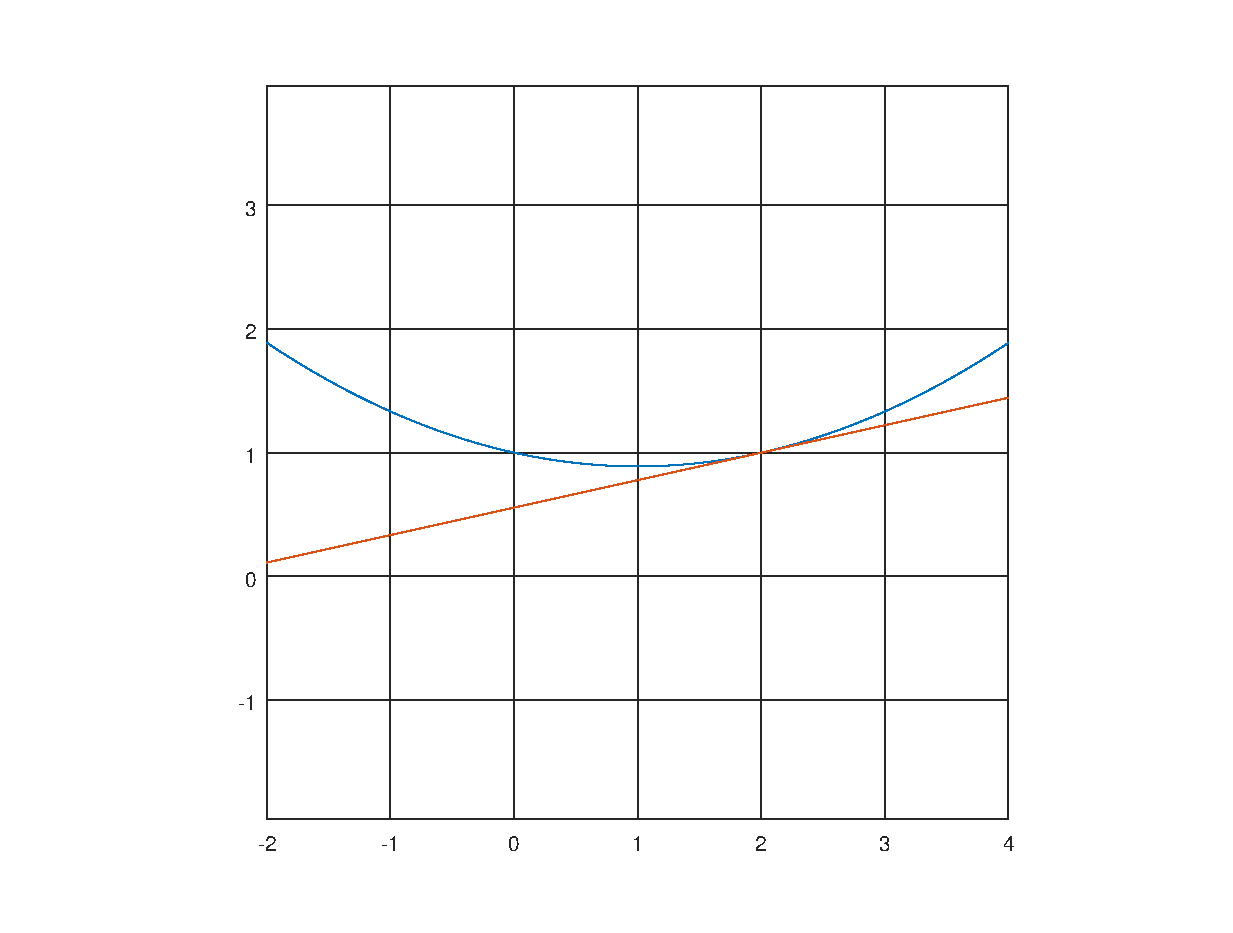
\includegraphics{1-1.eps}
            }
        \end{center}
        \caption{運用例}
        \label{fig:1-1}
    \end{figure}






%\end{document}
